\chapter{Конструкторский раздел}

\section{Формализация сущностей системы}

На основе выделенных ранее сущностей спроектированы следующие таблицы базы данных.

	 Таблица Users содержит данные о пользователях системы. Включает следующие поля:
	\begin{itemize}
            \item id -- целое число, идентификатор пользователя;
		\item name -- строка, имя пользователя;
		\item login, password -- строки, логин и пароль пользователя;
            \item role -- целое число, роль пользователя ссылается на таблицу Roles.
	\end{itemize}

    Таблица Ratings содержит информацию, присущую лишь участникам и капитанам команд. Включает в себя поля part\_id -- целое число, идентификатор пользователя из таблицы Users, и rating -- целое число, рейтинг пользователя.
 
	    Таблица Hackathons -- содержит информацию о хакатонах. Включает следующие поля:
	\begin{itemize}
            \item id -- целое число, идентификатор хакатона;
            \item name -- строка, название хакатона;
            \item address -- строка, адрес места проведения хакатона; 
		\item date --  тип <<Дата и время>>, дата проведения хакатона;
		\item theme -- строка, тематика хакатона;
            \item duration -- вещественное число, продолжительность хакатона в часах. 
            \item id\_first, id\_second, id\_third -- целые числа, id команд занявших первое, второе и третье место соответственно.
	\end{itemize}
        
	     Таблица Requests -- содержит информацию о заявках системы. Включает следующие поля:
	\begin{itemize}
		\item id -- целое число, идентификатор заявки;
		\item type -- целое число, тип заявки; 
		\item requester\_id -- id пользователя, подавшего заявку;
		\item name -- название команды / мероприятия, опциональное поле;
		\item comment -- комментарий заявки;
		\item adm\_id -- id администратора, закрывшего заявку;
		\item status -- статус заявки.
	\end{itemize}
 
	 Таблица Teams -- содержит информацию о командах. Включает следующие поля:
	\begin{itemize}
		\item id -- целое число, идентификатор команды;
		\item name -- строка, название команды;
            \item rating -- целое число, рейтинг команды - является суммой рейтингов всех участников команды;
            \item cap\_id -- целое число, id капитана команды.
	\end{itemize}

    Кроме того, были спроектированы следующие вспомогательные таблицы: 
    \begin{itemize}
        \item таблица Statuses, содержащая идентификаторы возможных статусов заявок, в которой записи полями id,
        принимающими значения 1, 2, 3, 4 обозначают статусы <<Открыта>>, <<В работе>>, <<Принята>> и <<Отклонена>> соответственно;
        \item таблица RequestTypes, содержащая идентификаторы типов заявок, содержит записи со следующими id 1, 2, 3, 4, обозначающими "Создание команды", "Создание события", "Присоединение к команде", "Присоединение к событию";
        \item таблица Roles, содержащая идентификаторы возможных ролей пользователей.
    \end{itemize}

    
Соответствующая диаграмма по описанным выше данным представлена на рисунке \ref{er}.

\begin{figure}[H]
	\begin{center}
		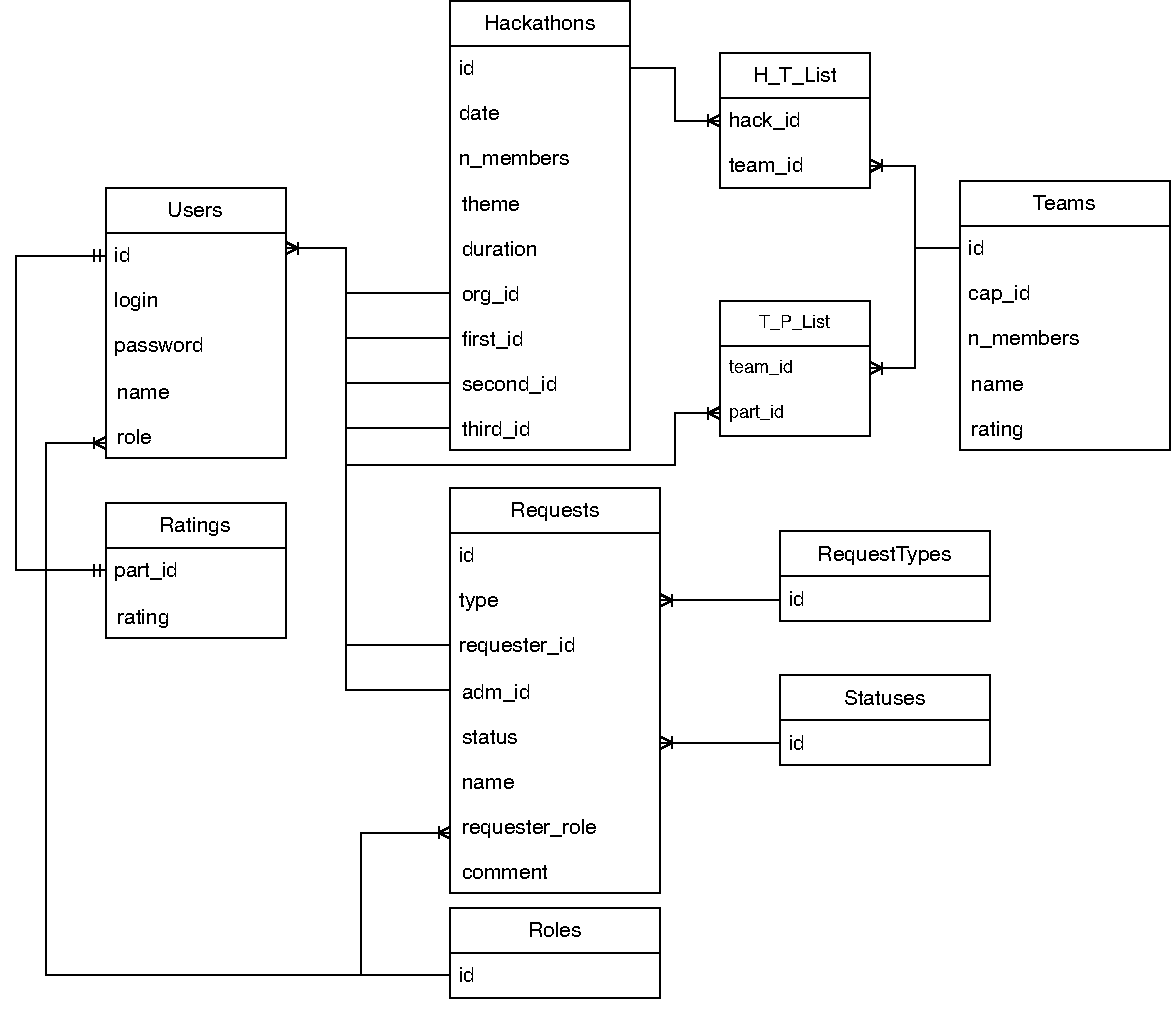
\includegraphics[page=1,scale=0.8]{assets/db_er.drawio.pdf}
	\end{center}
	\caption{Схема базы данных}
	\label{er}
\end{figure}

\section{Ролевая модель}

Для обеспечения корректной работы пользователей с системой на уровне базы данных выделена следующая ролевая модель.

\begin{enumerate}
	\item Participant -- участник хакатона. Обладает правом SELECT над таблицами Users, Teams, Hackathons, H\_T\_List и T\_P\_List, Ratings, а также правом INSERT/UPDATE  над таблицей Requests.
        \item Captain -- капитан команды, обладает всеми правами пользователя \newline
        Participant и правами UPDATE над таблицей Teams.
        \item Organizer -- организатор хакатона. Обладает всеми правами пользователя Participant, а также правами UPDATE/DELETE над таблицей Hackathons.
	\item Administrator -- администратор. обладает всеми правами над всеми таблицами.
 
\end{enumerate}

Использование ролевой модели на уровне базы данных гарантирует безопасность доступа к объектам.

\section{Триггер}

В системе предусмотрен механизм обновления рейтинга участников и команд, в которых они состоят. Он реализован также триггером AFTER на действие UPDATE в таблицу Hackathons. Данный триггер при обновлении записи хакатона, увеличивает рейтинг участников команд, занявших первое, второе и третье место на 3, 2 и 1 соответственно. Кроме того, обновляется рейтинг команд, в которых состоят данные участнике

На рисунке \ref{trigger} представлена схема алгоритма работы выполняемой триггером функции updateRating().

\begin{figure}[H]
	\begin{center}
		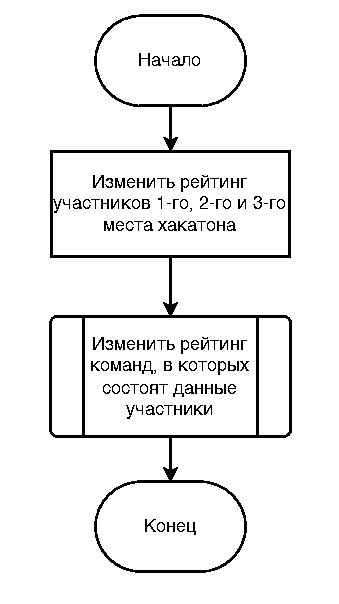
\includegraphics[page=1,scale=1]{assets/trigger.drawio.pdf}
	\end{center}
	\caption{Триггер AFTER для обновления рейтинга}
	\label{trigger}
\end{figure}

\section{Ограничения целостности базы данных}
В ходе проектирования базы данных были выделены следующие ограничения: 
\begin{itemize}
    \item логин и пароль пользователя должны содержать не больше 35 символов;
    \item рейтинг пользователя/команды - не может быть отрицательным;
    \item каждый участник может состоять только в одной команде;
    \item дата проведения добавляемого хакатона - не ранее завтрашнего дня от текущей даты;
    \item число участников в команде - не более пяти человек, включая капитана;
    \item число записей во вспомогательных таблицах Statuses, RequestTypes и Roles не может быть больше числа соответствующих сущностей.
\end{itemize}

\section{Вывод из раздела}

В данном разделе была произведена формализация сущностей системы с последующим составлением ролевой модели и выделением пользовательских прав, спроектированы основные и вспомогательные таблицы, построена ER-диаграмма базы данных, спроектирован триггер AFTER, обновляющий рейтинг участников и команд после обновления призовых мест хакатона, а также выделены ограничения целостности базы данных.